\section{
    Псевдорешение, алгоритм нахождения. Нормальное псевдорешение, алгоритм нахождения. Определение, смысл. Рассмотреть случаи для совместных и несовместных систем.
}

\subsection{
    Псевдорешение, алгоритм нахождения.
}

Рассмотрим СЛАУ 

$$A\vec{x} = \vec{b},$$

где $A$ - матрица размера $m \times n, \vec{x} \in \RR^n, \vec{b} \in \RR^m$. Каждому столбцу $\vec{x}$ можно сопоставить столбец $\vec{b} - A\vec{x}$, называемый \textit{вектором невязок}. Евклидову норму этого столбца $\norm{\vec{b} - A\vec{x}} = \sqrt{(\vec{b} - A\vec{x}, \vec{b} - A\vec{x})}$ называют \textit{нормой невязки}.

Для любой СЛАУ $A\vec{x} = \vec{b}$ найдется хотя бы один столбец $\vec{x}$, на котором норма невязки $v(x) = \norm{\vec{b} - A\vec{x}}$ принимает наименьшее значение $v_0$. Каждый такой столбец называется \textit{псевдорешением} СЛАУ $A\vec{x} = \vec{b}$. Итак,

\begin{definition}
    Вектор-столбец $\vec{x}$, такой, что норма невязки $\norm{\vec{b} - A\vec{x}}$ СЛАУ $A\vec{x} = \vec{b}$ принимает наименьшее значение, называется \textit{\textbf{псевдорешением}}.
\end{definition}

Если система совместна, то минимальное значение нормы невязки равно нулю и множество псевдорешений совпадает с множеством решений системы. Множество псевдорешений СЛАУ совпадает с множеством решений соответствующей \textit{нормальной системы} $A^TA\vec{x} = A^T\vec{b}$ (\textbf{*}см. 14 "билет"). 


\newpage


\subsection{
    Нормальное псевдорешение, алгоритм нахождения.
}


Среди всех псевдорешений СЛАУ $A\vec{x} = \vec{b}$ есть единственное псевдорешение, имеющее наименьшую норму. Оно называется \textit{нормальным}. Итак,

\begin{definition}
    Наименьшее по норме псевдорешение СЛАУ $A\vec{x} = \vec{b}$ называется \textbf{\textit{нормальным псевдорешением}}.
\end{definition}

Нормальное псевдорешение СЛАУ $A\vec{x} = \vec{b}$ является решением системы уравнений, которая получается, если к нормальной системе $A^TA\vec{x} = A^T\vec{b}$ добавить уравнения СЛАУ $F^T\vec{x} = \vec{0}$, где $F$ - матрица, составленная из столбцов ФСР СЛАУ $A\vec{x} = \vec{0}$.

\begin{equation*}
    \left(\begin{array}{c}
        A^TA \\
        F^T
    \end{array}\right)\vec{x}
    =
    \left(\begin{array}{c}
        A^T\vec{b} \\
        \vec{0}
    \end{array}\right)
.\end{equation*}


\newpage


\subsection{
    Пример для несовместной системы.
}

\begin{example}
    Рассмотрим простейшую систему

    \begin{equation}
        \begin{cases}
            x + y = 0 \\
            x + y = 1
        \end{cases}
    \end{equation}

    двух уравнений с двумя неизвестными. Видно, что эта система несовместна. Последовательно вычисляем

    \begin{equation}
        A = \left(\begin{array}{cc}
            1 & 1 \\
            1 & 1
        \end{array}\right), \thinspace \thinspace
        A^TA = \left(\begin{array}{cc}
            1 & 1 \\
            1 & 1
        \end{array}\right)^2 = \left(\begin{array}{cc}
            2 & 2 \\
            2 & 2
        \end{array}\right), \thinspace \thinspace
        A^Tb = \left(\begin{array}{cc}
            1 & 1 \\
            1 & 1
        \end{array}\right)\left(\begin{array}{c}
            0 \\
            1
        \end{array}\right) = \left(\begin{array}{c}
            1 \\
            1
        \end{array}\right)
    \end{equation}

    Таким образом, нормальная СЛАУ в этом случае состоит из двух одинаковых уравнений:

    \begin{equation}
        \begin{cases}
            2x + 2y = 1 \\
            2x + 2y = 1
        \end{cases}
    \end{equation}

    Множество решений нормальной системы, т.е. множество пар $x, y$, дающих минимальную невязку в исходной системе, на плоскости изображаются прямой $x + y = 0.5$ (рис. \ref{fig:picture_16_1}), а нормальным псевдорешением будет точка этой прямой, ближайшая к началу координат, т.е. точка с координатами $x = 0.25, y = 0.25$. Этой точке соответствует радиус-вектор с наименьшей нормой среди всех радиус-векторов точек прямой $x + y = 0.5$.
    
    К слову, если одно из уравнений исходной системы умножить на коэффициент, то и множество решений нормальной системы, и нормальное псевдорешение данной системы изменятся, так как умножение на коэффициент, вообще говоря, меняет его невязку.

    \begin{figure}[H]
        \centering
        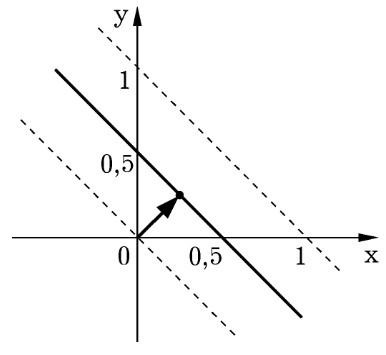
\includegraphics[scale=0.6]{images/16_1.jpg}
        \caption{}
        \label{fig:picture_16_1}
    \end{figure}

\end{example}
